\documentclass{article}

% % % % % % % % % % % % % % % % % % % % % % % % % % 
%
%				PACKAGES, SETTINGS & MACROS
%
% % % % % % % % % % % % % % % % % % % % % % % % % %

\usepackage{amsthm,amssymb,amsmath}
\usepackage[numbers]{natbib}
\usepackage{algpseudocode}
\usepackage{tikz-network}
\usepackage{newfloat}
\usepackage{textcomp}
\usepackage{a4wide}
\usepackage{rotating}
\usepackage{booktabs}
\usepackage{xcolor}
\usepackage{lipsum}
\usepackage{xspace}

\definecolor{gray}{RGB}{66,66,66}
\definecolor{blue}{RGB}{27,72,105}
\definecolor{orange}{RGB}{255,139,0}
\usepackage[colorlinks=true,linkcolor={blue},citecolor={blue},urlcolor={blue}]{hyperref}

\DeclareFloatingEnvironment[fileext=loa,listname=List of Algorithms,name=Algorithm,placement=tbhp]{algorithm}

\theoremstyle{definition}
\newtheorem{definition}{Definition}
\newtheorem{theorem}{Theorem}
\newtheorem{corollary}[theorem]{Corollary}
\newtheorem{lemma}[theorem]{Lemma}

\newcommand{\secref}[1]{Section~\ref{sec:#1}\xspace}
\newcommand{\figref}[1]{Fig.~\ref{fig:#1}\xspace}
\newcommand{\subfigref}[2]{Fig.~\ref{fig:#1}#2\xspace}
\newcommand{\tblref}[1]{Table~\ref{tbl:#1}\xspace}
\renewcommand{\eqref}[1]{Eq.~(\ref{eq:#1})\xspace}
\renewcommand{\algref}[1]{Algorithm~\ref{alg:#1}\xspace}
\newcommand{\theref}[1]{Theorem~\ref{the:#1}\xspace}
\newcommand{\therefs}[2]{Theorems~\ref{the:#1} and~\ref{the:#2}\xspace}

\DeclareMathOperator*{\argmin}{arg\,min}
\renewcommand{\O}{\mathcal{O}}

\newcommand{\refs}{{\bf\color{orange}[REFS]}}
\newcommand{\todo}{{\bf\color{orange}TODO}}
\newcommand{\lips}[1]{{\bf\color{orange}TEXT}~\emph{\color{gray}\lipsum[#1]}}
\newcommand{\redo}[1]{{\bf\color{orange}REDO}~{\color{blue}#1}}

\newcommand{\stnode}[3]{\Vertex[x=#1,y=#2,color={27,72,105},opacity=0.5,RGB,Math,IdAsLabel]{#3}}
\newcommand{\ijknode}[3]{\Vertex[x=#1,y=#2,size=0.5,color={255,139,0},opacity=1,RGB,Math,IdAsLabel]{#3}}
\newcommand{\xnode}[4]{\Vertex[x=#1,y=#2,size=#3,color={255,139,0},opacity=1,RGB,Math,IdAsLabel]{#4}}
\newcommand{\lnode}[4]{\Vertex[x=#1,y=#2,size=0.5,color=white,Math,label=#4]{#3}}
\newcommand{\enode}[3]{\Vertex[x=#1,y=#2,size=0.5,color=white,Math,IdAsLabel]{#3}}
\newcommand{\anode}[3]{\Vertex[x=#1,y=#2,size=0.4,color=white,Math]{#3}}
\newcommand{\pledge}[2]{\Edge[lw=0.8,color=black,Direct,Math,label=p](#1)(#2)}
\newcommand{\pedge}[2]{\Edge[lw=1,color=black,Direct,Math,label=p](#1)(#2)}
\newcommand{\xedge}[3]{\Edge[lw=1,color=black,distance=0.4,Direct,Math,label=#3](#1)(#2)}
\newcommand{\eedge}[2]{\Edge[lw=1,color=black,Direct,Math](#1)(#2)}

\graphicspath{{figures/}}

% % % % % % % % % % % % % % % % % % % % % % % % % % 
%
%			TITLE, AUTHORS & AFFILIATIONS
%
% % % % % % % % % % % % % % % % % % % % % % % % % %

\title{Intermediacy of publications}
\author{Lovro \v{S}ubelj$^1$, Ludo Waltman$^2$, Nees Jan van Eck$^2$ \& Vincent Traag$^2$}
\date{\small $^1$University of Ljubljana, Faculty of Computer and Information Science, Ljubljana, Slovenia\\
$^2$Leiden University, Centre for Science and Technology Studies, Leiden, Netherlands}
\begin{document}

\maketitle

% % % % % % % % % % % % % % % % % % % % % % % % % % 
%
%				ABSTRACT
%
% % % % % % % % % % % % % % % % % % % % % % % % % %

\begin{abstract}
	\lips{1}
\end{abstract}

% % % % % % % % % % % % % % % % % % % % % % % % % % 
%
%				INTRODUCTION
%
% % % % % % % % % % % % % % % % % % % % % % % % % %

\section{\label{sec:introduction}Introduction}

At the interface between the fields of scientometrics and network analysis, many approaches have been developed for studying the structure and development of the scientific literature in a specific research area or on a specific research topic. Clustering techniques, also known as community detection techniques, have been applied to scientometric networks in order to identify clusters of closely related publications or journals~\citep[e.g.,][]{Boyack2010,Rosvall2008,Waltman2012}. Such clusters can be considered to represent research areas. Clustering techniques have for instance been employed to identify emerging research areas~\cite{Small2014,Wang2018}. Visualization tools have been used to visually represent the structure and development of the literature in a research area, focusing either on visualizations of scientometric networks in general~\cite{Chen2006,VanEck2010} or specifically on visualizations of citation networks of publications~\cite{Garfield2003,VanEck2014}. Centrality measures have also frequently been applied to scientometric networks, for instance to study the interdisciplinarity of journals~\cite{Leydesdorff2007} or the influence of authors~\cite{Newman2001}. Various approaches have also been introduced specifically for analyzing citation networks of publications. These for instance include main path analysis~\cite{Hummon1989} and transitive reduction~\cite{Clough2015}.

In this paper, we introduce a new approach for analyzing citation networks of publications. We propose an indicator called intermediacy. Given two publications dealing with a specific research topic, an older publication and a more recent one, intermediacy can be used to identify publications that appear to play a major role in the intellectual development from the older to the more recent publication. These are publications that, based on citation links, are important in connecting the older and the more recent publication.

Intermediacy somewhat resembles the idea of main path analysis, originally proposed by~\citet{Hummon1989}. However, as we will make clear, there are fundamental differences between intermediacy and main path analysis. Most significantly, we will show that main path analysis tends to favor longer citation paths over shorter ones, whereas intermediacy has the opposite tendency. For the purpose of tracing intellectual developments in the scientific literature, we argue that intermediacy yields better results than main path analysis.

This paper is organized as follows. In~\secref{intermediacy}, we define intermediacy, we study the mathematical properties of intermediacy, and we describe algorithms for calculating intermediacy. In~\secref{empirical}, we present two cases that provide empirical illustrations of the use of intermediacy. We discuss our conclusions in~\secref{conclusions}.

% % % % % % % % % % % % % % % % % % % % % % % % % % 
%
%				INTERMEDIACY
%
% % % % % % % % % % % % % % % % % % % % % % % % % %

\section{\label{sec:intermediacy}Intermediacy}

Consider a directed acyclic graph $G = (V, E)$, where $V$ denotes the set of nodes of $G$ and $E$ denotes the set of edges of $G$. The edges are directed. A certain node $s \in V$ is referred to as the source, while another node $t \in V$ is referred to as the target. We assume that each node $v \in V$ is located on a path from the source $s$ to the target $t$. We refer to such a path as a source-target path.

\begin{definition}
	Given a source $s$ and a target $t$, a path from $s$ to $t$ is called a \emph{source-target path}.
\end{definition}

Informally, the more important the role of a node $v \in V$ in connecting the source $s$ to the target $t$, the higher the intermediacy of $v$. To define the concept of intermediacy in a formal way, we assume that each edge $e \in E$ is active with a certain probability. We assume the probability of being active to be the same for all edges $e \in E$. This probability is denoted by $p$. The probability of an edge being inactive is denoted by $q = 1 – p$. Based on the idea of active and inactive edges, the following definitions can be introduced.

\begin{definition}
	If all edges on a path are active, the path is called \emph{active}. Otherwise the path is called \emph{inactive}. If a node $v \in V$ is located on an active source-target path, the node is called \emph{active}. Otherwise the node is called \emph{inactive}.
\end{definition}

For two nodes $u, v \in V$, we use $X_{uv}$ to indicate whether there is an active path from node $u$ to node $v$ ($X_{uv} = 1$) or not ($X_{uv} = 0$). The probability that there is an active path from node $u$ to node $v$ is denoted by $\Pr(X_{uv} = 1)$. We use $X_{st}(v)$ to indicate whether there is an active source-target path that goes through node $v$ ($X_{st}(v) = 1$) or not ($X_{st}(v) = 0$). The probability that there is an active source-target path that goes through node $v$ is denoted by $\Pr(X_{st}(v) = 1)$. Note that this probability equals the probability that node $v$ is active.

The concept of intermediacy can now be defined as follows.

\begin{definition}
	The \emph{intermediacy} $\phi_v$ of a node $v \in V$ equals the probability that $v$ is active, that is, $\phi_v = \Pr(X_{st}(v) = 1)$.
\end{definition}

\subsection{\label{sec:properties}Properties}

To get a better understanding of the notion of intermediacy, we study the properties of intermediacy in two limit cases. We first consider the limit case in which the probability $p$ of an edge being active tends to $0$. We then consider the limit case in which the probability $p$ tends to $1$. It turns out that a ranking of the nodes in a graph based on intermediacy has a natural interpretation in each of these limit cases.

Let $\ell_v$ denote the length of the shortest source-target path going through node $v \in V$. \theref{p0} presented below states that in the limit as the probability $p$ of an edge being active tends to $0$, the ranking of nodes based on intermediacy coincides with the ranking based on $\ell_v$, with nodes located on shorter source-target paths being more intermediate than nodes located on longer source-target paths.

The intuition for this result is as follows. When the probability of an edge being active is very close to $0$, almost all edges are inactive. Consequently, almost all source-target paths are inactive as well. However, from a relative point of view, longer source-target paths are much more likely to be inactive than shorter source-target paths. This mean that, again from a relative point of view, nodes located on shorter source-target paths have a much higher probability to be active than nodes located on longer source-target paths (even though for all nodes this probability is close to $0$). Nodes located on shorter source-target paths therefore have a higher intermediacy than nodes located on longer source-target paths.

\begin{theorem}
	In the limit as $p$ tends to $0$, $\ell_u < \ell_v$ implies $\phi_u > \phi_v$.
	\label{the:p0}
\end{theorem}

\begin{proof}
	Let $m = |E|$ denote the number of edges in the graph $G$. Suppose that the $m$ edges are split into two sets, one set of $M$ edges and another set of $m-M$ edges. The probability that the edges in the former set are all active while the edges in the latter set are all inactive equals
	$$P_M = p^M (1-p)^{m-M}.$$
	Consider a node $v \in V$. The shortest source-target path that goes through $v$ has a length of $\ell_v$. This means that at least $\ell_v$ edges need to be active in order to obtain an active source-target path that goes through $v$. Hence, the probability that there is an active source-target path that goes through $v$ can be written as
	$$\phi_v = \sum_{i = \ell_v}^m n_{vi} P_i,$$
	where $n_{vi} > 0$ for all $i = \ell_v,\dots,m$. Note that this probability equals the intermediacy of $v$.
	Now consider two nodes $u, v \in V$ with $\ell_u < \ell_v$. In the limit as $p$ tends to $0$, $\phi_u$ and $\phi_v$ both tend to $0$. However, they do so at different rates. More specifically, in the limit as $p$ tends to $0$, we have
	\begin{eqnarray}
		\phi_v / \phi_u & = & \left(\sum_{i = \ell_v}^m n_{vi} P_i\right) / \left(\sum_{i = \ell_u}^m n_{ui} P_i\right) \nonumber\\
		& = & \left(\sum_{i = \ell_v}^m n_{vi} P_i / P_{\ell_u}\right) / \left(\sum_{i = \ell_u}^m n_{ui} P_i / P_{\ell_u}\right) \nonumber\\
		& = & \left(\sum_{i = \ell_v}^m n_{vi} p^{i-\ell_u} (1-p)^{\ell_u-i}\right) / \left(\sum_{i = \ell_u}^m n_{ui} p^{i-\ell_u} (1-p)^{\ell_u-i}\right) \nonumber\\
		& = & 0 / n_{ui} \nonumber\\
		& = & 0.
	\end{eqnarray}
	Hence, in the limit as $p$ tends to $0$, $\phi_u > \phi_v$.
\end{proof}

Let $\sigma_v$ denote the number of edge independent source-target paths going through node $v \in V$. \theref{p1} presented below states that in the limit as the probability $p$ of an edge being active tends to $1$, the ranking of nodes based on intermediacy coincides with the ranking based on $\sigma_v$. The larger the number of edge independent source-target paths going through a node, the higher the intermediacy of the node.

The intuition for this result is as follows. When the probability of an edge being active is very close to $1$, almost all edges are active. Consequently, almost all source-target paths are active as well, and so are almost all nodes. A node is inactive only if all source-target paths going through the node are inactive. If there are $\sigma$ edge independent source-target paths that go through a node, this means that the node can be inactive only if there are at least $\sigma$ inactive edges. Consider two nodes $u$ and $v$. Suppose that the number of edge independent source-target paths going through node $u$ is larger than the number of edge independent source-target paths going through node $v$. In order to be inactive, node $u$ then requires a larger number of inactive edges than node $v$. Since the probability of an edge being active is very close to $1$, this means that, from a relative point of view, node $u$ has a much lower probability of being inactive than node $v$ (even though for both nodes this probability is close to $0$). Hence, node $u$ has a higher intermediacy than node $v$. More generally, nodes located on a larger number of edge independent source-target paths have a higher intermediacy than nodes located on a smaller number of edge independent source-target paths.

\begin{theorem}
	In the limit as $p$ tends to $1$, $\sigma_u > \sigma_v$ implies $\phi_u > \phi_v$.
	\label{the:p1}
\end{theorem}

\begin{proof}
	Let $m = |E|$ denote the number of edges in the graph $G$. Suppose that the $m$ edges are split into two sets, one set of $M$ edges and another set of $m-M$ edges. The probability that the edges in the former set are all inactive while the edges in the latter set are all active equals
	$$Q_M = q^M(1-q)^{m-M}.$$
	Consider a node $v \in V$. There are $\sigma_v$ edge independent source-target paths that go through $v$. This means that at least $\sigma_v$ edges need to be inactive in order for there to be no active source-target path that goes through $v$. Hence, the probability that there is no active source-target path that goes through $v$ can be written as
	$$\Phi_v = \sum_{i = \sigma_v}^m n_{vi} Q_i,$$
	where $n_{vi} > 0$ for all $i = \sigma_v,\dots,m$. Note that the intermediacy of $v$ equals $1$ minus the above probability, that is, $\phi_v = 1-\Phi_v$.
	Now consider two nodes $u, v \in V$ with $\sigma_u > \sigma_v$. In the limit as $p$ tends to $1$, $\Phi_u$ and $\Phi_v$ both tend to $0$. However, they do so at different rates. More specifically, in the limit as $p$ tends to $1$, we have
	\begin{eqnarray}
		\Phi_u / \Phi_v & = & \left(\sum_{i = \sigma_u}^m n_{ui} Q_i\right) / \left(\sum_{i = \sigma_v}^m n_{vi} Q_i\right) \nonumber\\
		& = & \left(\sum_{i = \sigma_u}^m n_{ui} Q_i / Q_{\sigma_v}\right) / \left(\sum_{i = \sigma_v}^m n_{vi} Q_i / Q_{\sigma_v}\right) \nonumber\\
		& = & \left(\sum_{i = \sigma_u}^m n_{ui} q^{i-\sigma_v} (1-q)^{\sigma_v-i}\right) / \left(\sum_{i = \sigma_v}^m n_{vi} q^{i-\sigma_v} (1-q)^{\sigma_v-i}\right) \nonumber\\
		& = & 0 / n_{vi} \nonumber\\
		& = & 0.
	\end{eqnarray}
	Hence, in the limit as $p$ tends to $1$, $\Phi_u < \Phi_v$, which implies that $\phi_u > \phi_v$.
\end{proof}

\therefs{p0}{p1} are concerned with the properties of intermediacy in the limit cases in which the probability $p$ of an edge being active tends to either $0$ or $1$. \subfigref{examples}{A} provides some insight into the behavior of intermediacy for values of the probability $p$ that are in between these two extremes. The figure shows two graphs. In the left graph, there is a direct path from node $u$ to node $v$. There are no indirect paths. In this graph, the probability that there is an active path from $u$ to node $v$ equals $p$. In the right graph, there is no direct path from node $u$ to node $v$. However, there are $k$ indirect paths of length $2$. Each of these paths has a probability of $p^2$ of being active. Consequently, the probability that there is at least one active path from node $u$ to node $v$ equals $1-(1-p^2)^k$. The table shown in \subfigref{examples}{A} presents for different values of $k$ the value of $p$ for which the probability that there is an active path from node $u$ to node $v$ is the same in the left and the right graph. For instance, suppose that $k = 5$ and $p = 0.22$. Clearly, in the left graph, the probability that there is an active path from node $u$ to node $v$ then equals $0.22$. However, in the right graph, this probability also equals $0.22$, since $1-(1-p^2)^k = 0.22$. In other words, when the probability $p$ of an edge being active is set to $0.22$, a direct path between two nodes is considered equally strong as $5$ indirect paths of length $2$. Likewise, the table for instance indicates that for $p = 0.62$ a direct path between two nodes is considered equally strong as $2$ indirect paths of length $2$. Based on \subfigref{examples}{A}, one can choose a value for the probability $p$ that one considers appropriate for a particular analysis.

\begin{figure}[t]
   \centering%
   \begin{minipage}{0.4\textwidth}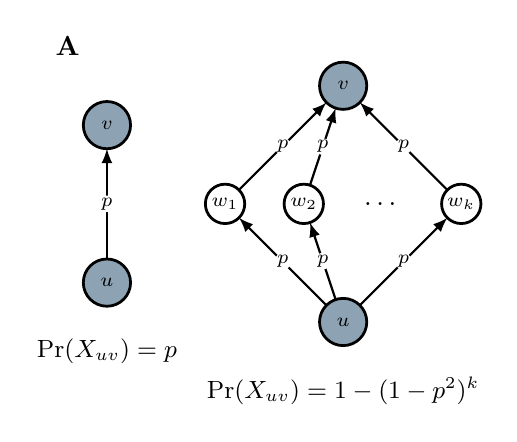
\begin{tikzpicture}
	\stnode{0}{0.5}{u} \stnode{0}{2.5}{v}
	\pledge{u}{v}
	\stnode{3}{0}{u} \stnode{3}{3}{v}
	\enode{1.5}{1.5}{w_1} \enode{2.5}{1.5}{w_2} \enode{4.5}{1.5}{w_k}
	\pledge{u}{w_1} \pledge{u}{w_2} \pledge{u}{w_k}
	\pledge{w_1}{v} \pledge{w_2}{v} \pledge{w_k}{v}	
	\draw (-0.5,3.5) node {{\bf A}} (3.5,1.5) node {\dots}; 
	\draw (0,-0.375) node {{\small$\Pr(X_{uv})=p$}} (3,-0.875) node {{\small$\Pr(X_{uv})=1-(1-p^2)^k$}};
   \end{tikzpicture}\end{minipage}%
   \begin{minipage}{0.2\textwidth}\hskip8pt\begin{tabular}{cc}
	$k$ & $p$ \\\midrule
	$2$ & $0.62$ \\
	$3$ & $0.39$ \\
	$4$ & $0.28$ \\
	$5$ & $0.22$ \\
	$6$ & $0.18$ \\
	$7$ & $0.15$ \\
	$8$ & $0.13$ \\
	$9$ & $0.12$ \\
	$10$ & $0.11$ \\
   \end{tabular}\end{minipage}%
   \begin{minipage}{0.4\textwidth}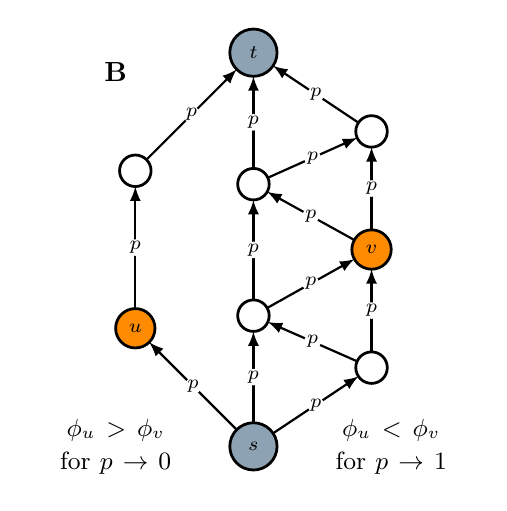
\begin{tikzpicture}
   	\stnode{0}{-1}{s} \stnode{0}{4}{t}
	\ijknode{-1.5}{0.5}{u} \ijknode{1.5}{1.5}{v}
	\anode{1.5}{0}{k1} \anode{0}{0.66}{l1}
	\anode{1.5}{3}{k2} \anode{0}{2.33}{l2}
	\anode{-1.5}{2.5}{k3}
	\pledge{s}{u} \pledge{u}{k3} \pledge{k3}{t}
	\pledge{s}{k1} \pledge{s}{l1}
	\pledge{k1}{v} \pledge{l1}{v} 
	\pledge{v}{k2} \pledge{v}{l2}
	\pledge{k2}{t} \pledge{l2}{t} 
	\pledge{l1}{l2} \pledge{k1}{l1} \pledge{l2}{k2}
	\draw (-1.75,3.75) node {{\bf B}}; 
	\draw (-1.75,-1) node[text width=2cm,align=center] {{\small$\phi_u>\phi_v$ for $p\to 0$}};
	\draw (1.75,-1) node[text width=2cm,align=center] {{\small$\phi_u<\phi_v$ for $p\to 1$}};
   \end{tikzpicture}\end{minipage}
   \vskip8pt\resizebox{0.7\textwidth}{!}{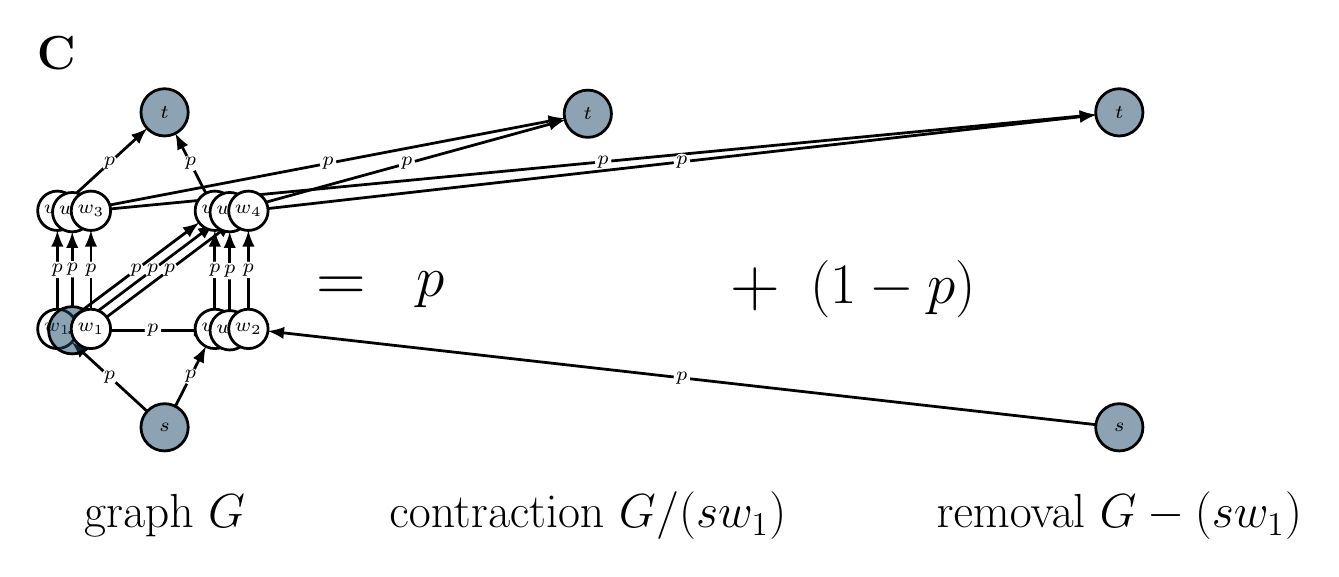
\begin{tikzpicture}
   	\def\x{0.375} \def\y{0}
	\stnode{\x}{\y}{s} \stnode{\x}{\y+4}{t}
	\enode{\x-1}{\y+1.25}{w_1} \enode{\x-1}{\y+2.75}{w_3} 
	\enode{\x+1}{\y+1.25}{w_2} \enode{\x+1}{\y+2.75}{w_4}
	\pedge{s}{w_1} \pedge{w_1}{w_3} \pedge{w_3}{t}
	\pedge{s}{w_2} \pedge{w_2}{w_4} \pedge{w_4}{t} \pedge{w_1}{w_4}
	\draw (\x,\y-1.125) node {{\LARGE graph $G$}};
	\draw (\x+2.25,\y+1.75) node {{\Huge$=$}};
	\def\x{5.75} \def\y{-0.5}
	\stnode{\x-1}{\y+1.25}{s} \stnode{\x}{\y+4}{t}
	\enode{\x-1}{\y+2.75}{w_3} 
	\enode{\x+1}{\y+1.25}{w_2} \enode{\x+1}{\y+2.75}{w_4}
	\pedge{s}{w_3} \pedge{w_3}{t}
	\pedge{s}{w_2} \pedge{w_2}{w_4} \pedge{w_4}{t} \pedge{s}{w_4}
	\draw (\x,\y-0.625) node {{\LARGE contraction $G/(sw_1)$}};
	\draw (\x-2.0,\y+2.25) node {{\huge$p$}};
	\draw (\x+2.125,\y+2.25) node {{\Huge$+$}};
	\def\x{12.5} \def\y{0}
	\stnode{\x}{\y}{s} \stnode{\x}{\y+4}{t}
	\enode{\x-1}{\y+1.25}{w_1} \enode{\x-1}{\y+2.75}{w_3} 
	\enode{\x+1}{\y+1.25}{w_2} \enode{\x+1}{\y+2.75}{w_4}
	\pedge{w_1}{w_3} \pedge{w_3}{t}
	\pedge{s}{w_2} \pedge{w_2}{w_4} \pedge{w_4}{t} \pedge{w_1}{w_4}
	\draw (\x,\y-1.125) node {{\LARGE removal $G-(sw_1)$}};
	\draw (\x-2.875,\y+1.75) node {{\huge$(1-p)$}};
	\draw (-1,4.75) node {{\bf\LARGE C}}; 
   \end{tikzpicture}}
   \vskip8pt\resizebox{0.99\textwidth}{!}{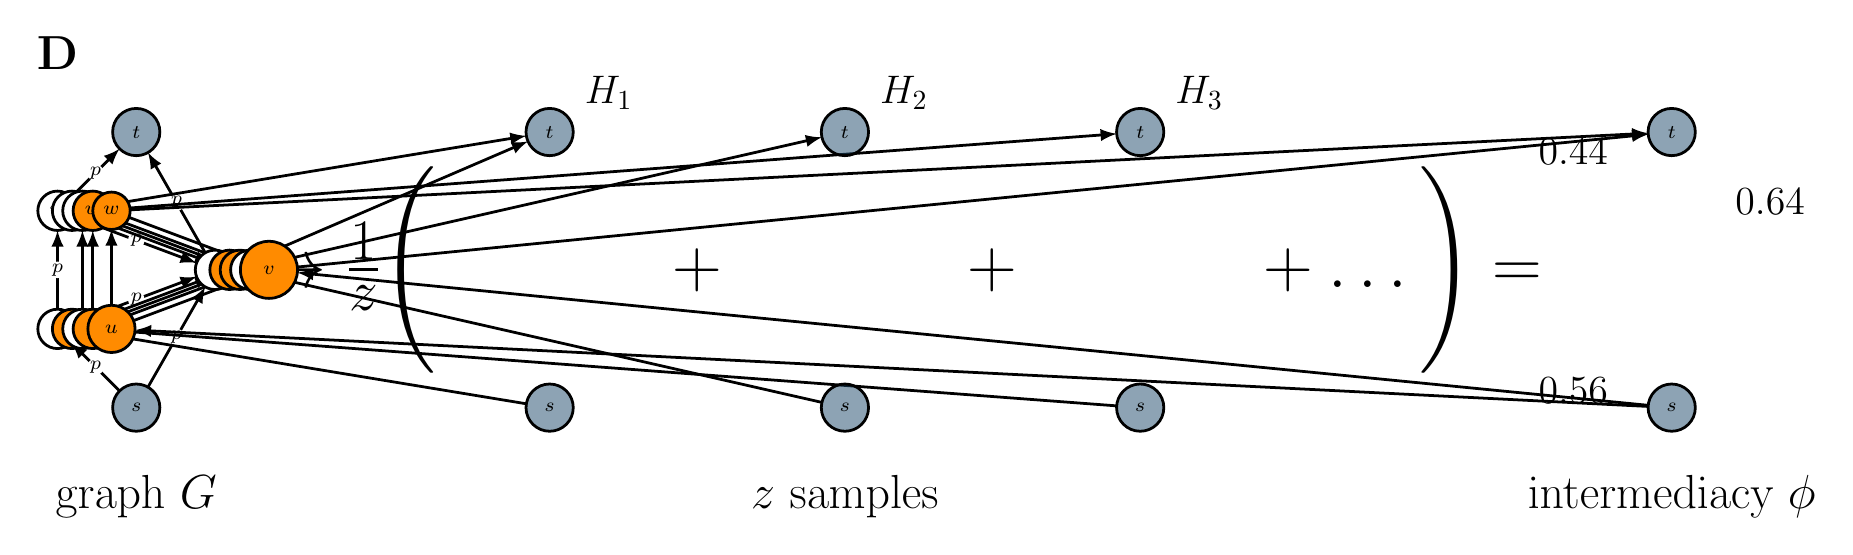
\begin{tikzpicture}
   	\def\x{0}
	\stnode{\x}{0}{s} \stnode{\x}{3.5}{t}
	\enode{\x-1}{1}{u} \enode{\x-1}{2.5}{w} \enode{\x+1}{1.75}{v}
	\pedge{s}{u} \pedge{u}{w} \pedge{w}{t}
	\pedge{s}{v} \pedge{v}{t} \pedge{u}{v} \pedge{w}{v}
	\draw (\x,-1.125) node {{\LARGE graph $G$}};
	\draw (\x+2.675,1.75) node {{\Huge$\rightarrow\frac{1}{z}\Bigg($}};
	\def\x{5.25}
	\stnode{\x}{0}{s} \stnode{\x}{3.5}{t}
	\ijknode{\x-1}{1}{u} \enode{\x-1}{2.5}{w} \ijknode{\x+1}{1.75}{v}
	\eedge{s}{u} \eedge{w}{t} 
	\eedge{v}{t} \eedge{u}{v} \eedge{w}{v}
	\draw (\x+0.75,4) node {{\Large $H_1$}};
	\draw (\x+1.875,1.75) node {{\Huge$+$}};
	\def\x{9}
	\stnode{\x}{0}{s} \stnode{\x}{3.5}{t}
	\enode{\x-1}{1}{u} \enode{\x-1}{2.5}{w} \ijknode{\x+1}{1.75}{v}
	\eedge{u}{w} 
	\eedge{s}{v} \eedge{v}{t} \eedge{u}{v} \eedge{w}{v}
	\draw (\x+0.75,4) node {{\Large $H_2$}};
	\draw (\x,-1.125) node {{\LARGE $z$ samples}};
	\draw (\x+1.875,1.75) node {{\Huge$+$}};
	\def\x{12.75}
	\stnode{\x}{0}{s} \stnode{\x}{3.5}{t}
	\ijknode{\x-1}{1}{u} \ijknode{\x-1}{2.5}{w} \enode{\x+1}{1.75}{v}
	\eedge{s}{u} \eedge{u}{w} \eedge{w}{t} 
	\eedge{u}{v} \eedge{w}{v} 
	\draw (\x+0.75,4) node {{\Large $H_3$}};
	\draw (\x+1.875,1.75) node {{\Huge$+$}};
	\def\x{16.5}
	\draw (\x,1.75) node {{\Huge$\dots\Bigg)=$}};
	\def\x{19.5}
	\stnode{\x}{0}{s} \stnode{\x}{3.5}{t}
	\xnode{\x-1}{1}{0.6}{u} \xnode{\x-1}{2.5}{0.475}{w} \xnode{\x+1}{1.75}{0.725}{v}
	\eedge{s}{u} \eedge{u}{w} \eedge{w}{t}
	\eedge{s}{v} \eedge{v}{t} \eedge{u}{v} \eedge{w}{v}
	\draw (\x-1.25,3.25) node {{\Large $0.44$}};
	\draw (\x-1.25,0.2125) node {{\Large $0.56$}};
	\draw (\x+1.25,2.6125) node {{\Large $0.64$}};
	\draw (\x,-1.125) node {{\LARGE intermediacy $\phi$}};
	\draw (-1,4.5) node {{\bf\LARGE D}}; 
   \end{tikzpicture}}
   \caption{\redo{Toy examples, asymptotic properties and algorithms' details.}}
   \label{fig:examples}
\end{figure}

\subsection{Algorithms}

\redo{Although the problem is NP-hard~\cite{Johnsona} we have devised an exact algorithm that is relatively efficient. 
Nonetheless, the algorithm is exact and has an exponential runtime.
This implies that the exact algorithm can only be used on relatively small datasets.
We therefore also propose a straightforward Monte Carlo algorithm to approximate the intermediacy.}

\subsection{Exact algorithm}

\redo{The exact algorithm is based on contraction and deletion of edges.
The basis of this algorithm is the fact that the probability there is a path between two nodes $i$ and $j$ can be decomposed as follows~\cite{Johnsona}
\begin{equation}
	\Pr(X_{ij} = 1 \mid G) = (1 - q) \Pr(X_{ij} = 1 \mid G/e) + q \Pr(X_{ij} = 1 \mid G - e)
\label{eq:recursive_path_prob}
\end{equation}
where $G/e$ denotes contraction of edge $e$ (in which it is assumed that $e$ itself is also deleted, and does not remain as a self-loop) and $G - e$ the deletion of edge $e$.
\eqref{eq:recursive_path_prob} yields a straightforward recursive method to calculate $\Pr(X_{ij} = 1)$ which can then easily be used to calculate $\Pr(X_{st}(i) = 1)$ using \eqref{eq:decompose_intermediacy}.
However, given a contracted graph $G/e$ we can also calculate the probability for some other pair of nodes, rather than only for the pair $ij$.}

\redo{Note that we are interested in the path probabilities $X_{si}$ for all $i$, but that the source $s$ is fixed.
If we contract some edge $(si)$ we then know that $\Pr(X_{si} = 1 \mid G/(si)) = 1$.
Hence, 
\begin{equation}
  \Pr(X_{si} = 1 \mid G) = (1 - q) + q \Pr(X_{si} = 1 \mid G - (si)).
\end{equation}
Since we are only interested in path probabilities $X_{si}$ we can always contract towards the source node $s$.
If we keep track of the probability of the state of contraction/deletion, we can rely on that to calculate the probability once we contract an edge.
If we denote this probability with $r$, we can thus add $r(1 - q)$ to the probability $\Pr(X_{si} = 1)$ if we contract the edge $(si)$.}

\redo{Note that we can follow the exact same procedure for the target if we reverse the direction of the graph $G$.
Let us denote the reverse of the edge direction of the edges with $E^T$, in line with the transpose of the adjacency matrix.}

\redo{Finally, there is a tricky thing of dealing with multiple parallel edges.
In order to deal with this, multiple parallel edges have to be combined into a single edge, and the failure probability of the combined edge is the product of the failure probability of the parallel edges.
For example, if there are two parallel edges that fail with probability $q$, the probability that the combined edge fails is then $q^2$.
This simply implies that the combined edge fails if all individual edges fail.
We hence have to maintain the failure probability on an edge basis, so that edge $e$ has failure probability $q_e$.
This also immediately yields an algorithm that in principle is suited for working with different failure probability for different edges.
The operation $G/e$ is assumed to perform also this combining of parallel edges.}

\redo{Our exact algorithm is summarised in Algorithm~\ref{alg:exact}.
Note that the pseudo-code of this algorithm uses explicit contraction, whereas in practice we rely on implicit contraction.
Although implicit contraction is more efficient, is clutters the pseudo-code too much.
Note that in practice, we limit $G$ to those nodes that are intermediate to $s$ and $t$, since the intermediacy of any other nodes is $0$ by definition.
However, to keep the pseudo-code clean, we have not included this in the pseudo-code.}

\begin{algorithm}[bt]
  \begin{algorithmic}[1]
		\Function{Intermediacy}{Graph $G$, Source $s$, Target $t$, Probability $q$}
      \State $X_{s} \gets $ \Call{PathProbabilities}{$G(V, E, q)$, $s$} 
      \State $X_{t} \gets $ \Call{PathProbabilities}{$(G(V, E^T, q)$, $t$}
			\State \Return $X_{s} X_{t}$ \Comment{Element-wise multiplication}
		\EndFunction
		\item[]
		\Function{PathProbabilities}{Graph $G(V,E,q)$, Source $s$, Probabilities $X=0$, StateProbability $r=1$}
		\If{$\{(s i) \in E\} \neq \emptyset$} \Comment{As long as we can contract}
			\State $e \gets \argmin_{(s i) \in E} i$ \Comment{Take the first edge}
			\State $i \gets \Call{Target}{$e$}$
			\If{$i \neq s$} \Comment{If not yet contracted}
				\State $X_i \gets X_i + r (1 - q_e)$
			\EndIf
			\State \Call{PathProbabilities}{$G/e$, $s$, $X$, $r (1 - q_e)$} \Comment{Contract edge $(i j)$}
			\State \Call{PathProbabilities}{$G-e$, $s$, $X$, $r q_e$} \Comment{Delete edge $(i j)$}
		\EndIf
		\State \Return $X$
		\EndFunction
	\end{algorithmic}
	\caption{\redo{Exact algorithm for calculating intermediacy.}}
	\label{alg:exact}
\end{algorithm}

\redo{The run-time of the function \textsc{PathProbabilities} in Algorithm~\ref{alg:exact} can easily be seen to be exponential.
For every edge $e \in E(G)$ there will be two recursive calls.
This will lead to $2^m$ function calls in total, where $m$ is the number of edges on paths between source $s$ and target $t$.
In order to approximate the intermediacy we will therefore rely on a Monte Carlo algorithm, which we will introduce in the next section.}

\subsection{Monte Carlo algorithm}

\redo{The Monte Carlo algorithm is very straightforward.
We will simply sample subgraphs $H$ and calculate whether a node $i$ lies on the path between $s$ and $t$.
Similar to the explanatory text in Section~\ref{sec:method}, we can define this as follows.
Let $P_{ij}$ be the indicator of whether edge $(ij) \in E$ fails or not, i.e. $P_{ij} = 1$ if $(ij)$ does not fail and $P_{ij} = 0$ if $(ij)$ does fail.
In other words, $\Pr(P_{ij} = 0) = q$ and $\Pr(P_{ij} = 1) = 1 - q$.
Then let $H$ be the subgraph of $G$ with edges $E' = \{ e \in E \mid P_{ij} = 1\}$.
These subgraphs $H$ are the subgraphs we sample in the Monte Carlo algorithm in Algorithm~\ref{alg:monte_carlo}.}

\begin{algorithm}[bt]
  \begin{algorithmic}[1]
		\Function{Intermediacy}{Graph $G$, Source $s$, Target $t$, Iterations $z$}
    \State \Return $\frac{1}{z} \sum_{k=1}^z \Pr(X_{st}(i) = 1 \mid H_k)$ % This is no longer a probability, right?
		\EndFunction
	\end{algorithmic}
	\caption{\redo{Monte Carlo algorithm for calculating intermediacy.}}
	\label{alg:monte_carlo}
\end{algorithm}

% % % % % % % % % % % % % % % % % % % % % % % % % % 
%
%				EMPIRICAL ILLUSTRATION
%
% % % % % % % % % % % % % % % % % % % % % % % % % %

\section{\label{sec:empirical}Empirical illustration}

We now present two cases that serve as empirical illustrations of the use of intermediacy. The first case deals with the topic of community detection and its relationship with scientometric research. This case was selected because we are well acquainted with the topic. The second case deals with the topic of peer review. This case is of interest because it was recently examined using main path analysis~\cite{Batagelj2017}. Hence, this case enables us to demonstrate the key differences between intermediacy and main path analysis.

\subsection{\label{sec:Q}Case 1: Community detection and scientometrics}

In the first case that we consider, we analyze how a method for community detection in networks ended up being used in the field of scientometrics to construct classification systems of scientific publications. In particular, we are interested in the development from Newman and Girvan (2004) to Klavans and Boyack (2017). These are our target and source publications. Newman and Girvan (2004) introduced a new metric for community detection in networks, known as modularity, while Klavans and Boyack (2017) compared different ways in which modularity-based approaches can be used to identify communities in citation networks.

Our analysis relies on data from the Scopus database produced by Elsevier. We also considered the Web of Science database produced by Clarivate Analytics. However, many citation links relevant for our analysis turned out to be missing in Web of Science. There are also missing citation links in Scopus, but for Scopus the problem seemed less significant than for Web of Science. This is why we work with Scopus. We refer to~\citet{VanEck2017} for a further discussion of the problem of missing citation links.

In the Scopus database, we found $n = 64\,223$ publications that are located on a citation path between our source and target publications. In total, we identified $m = 280\,033$ citation links between these publications. This means that on average each publication has $k = 2m / n = 8.72$ citation links, counting both incoming and outgoing links. We used our Monte Carlo algorithm to calculate the intermediacy of each publication for different values of the parameter $p$.

\figref{Q} presents some high-level results. The top-left plot shows how the probability of the existence of an active path between the source and target publications depends on the parameter $p$. This probability increases from a value of zero for $p = 0$ to a value close to one starting from $p = 0.25$. The vertical line indicates the value of $p$ obtained using the rule of thumb from percolation theory, as discussed in~\secref{intermediacy}. This rule of thumb yields $p = 1 / k = 0.11$, resulting in a probability of about $0.40$ for the existence of an active path between the source and target publications.

\begin{figure}[t]
  \centering%
  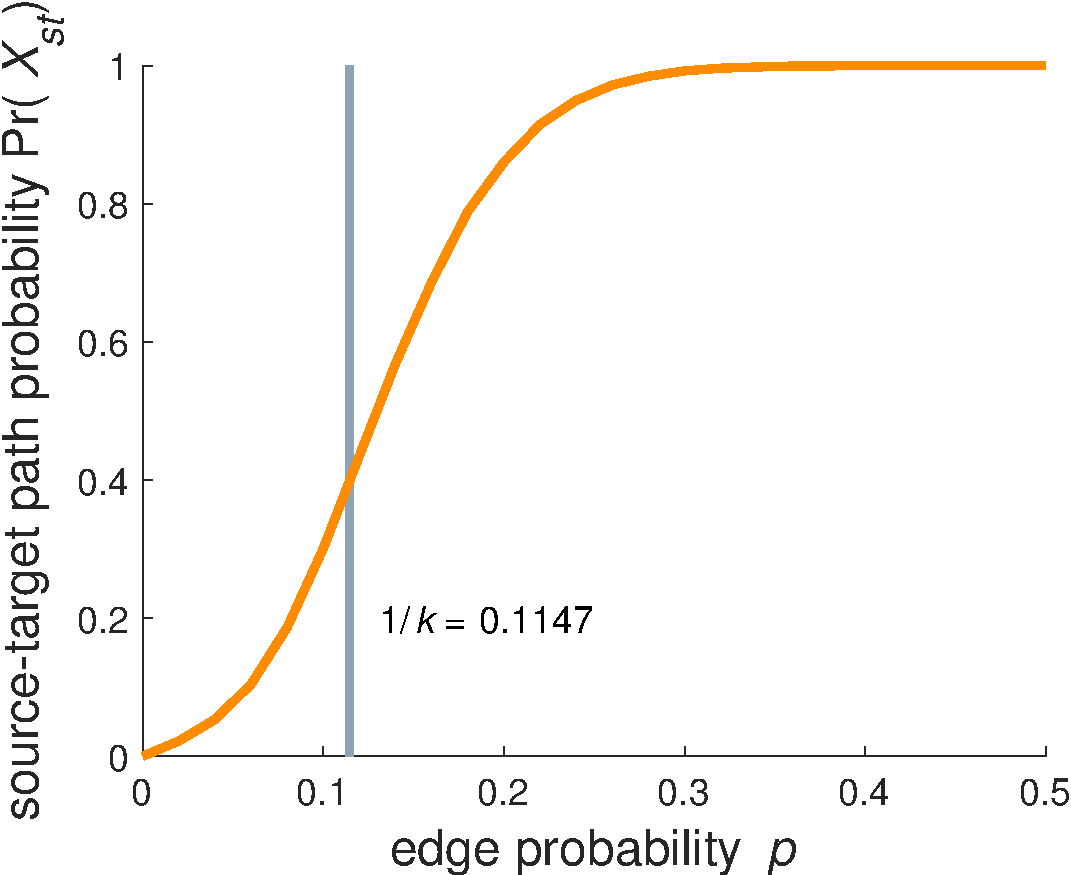
\includegraphics[width=0.4\textwidth]{phist_Q}\hskip0.075\linewidth
  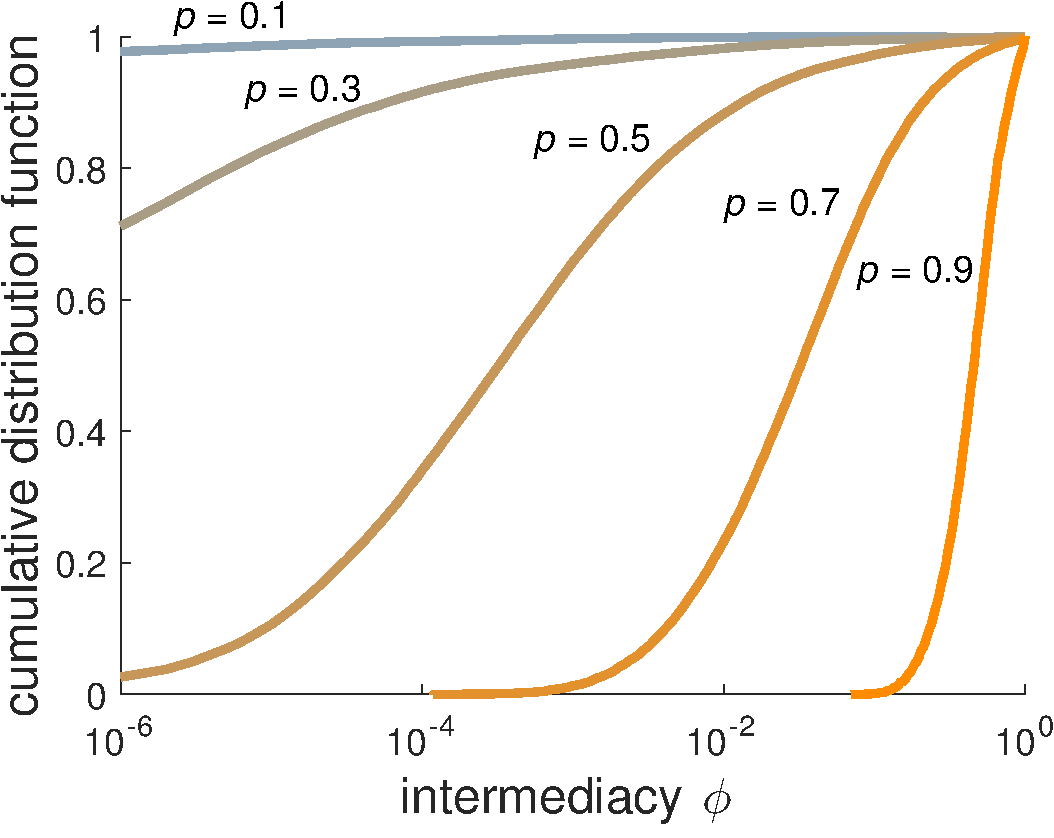
\includegraphics[width=0.4\textwidth]{distributions_Q}\\\vskip0.05\linewidth
  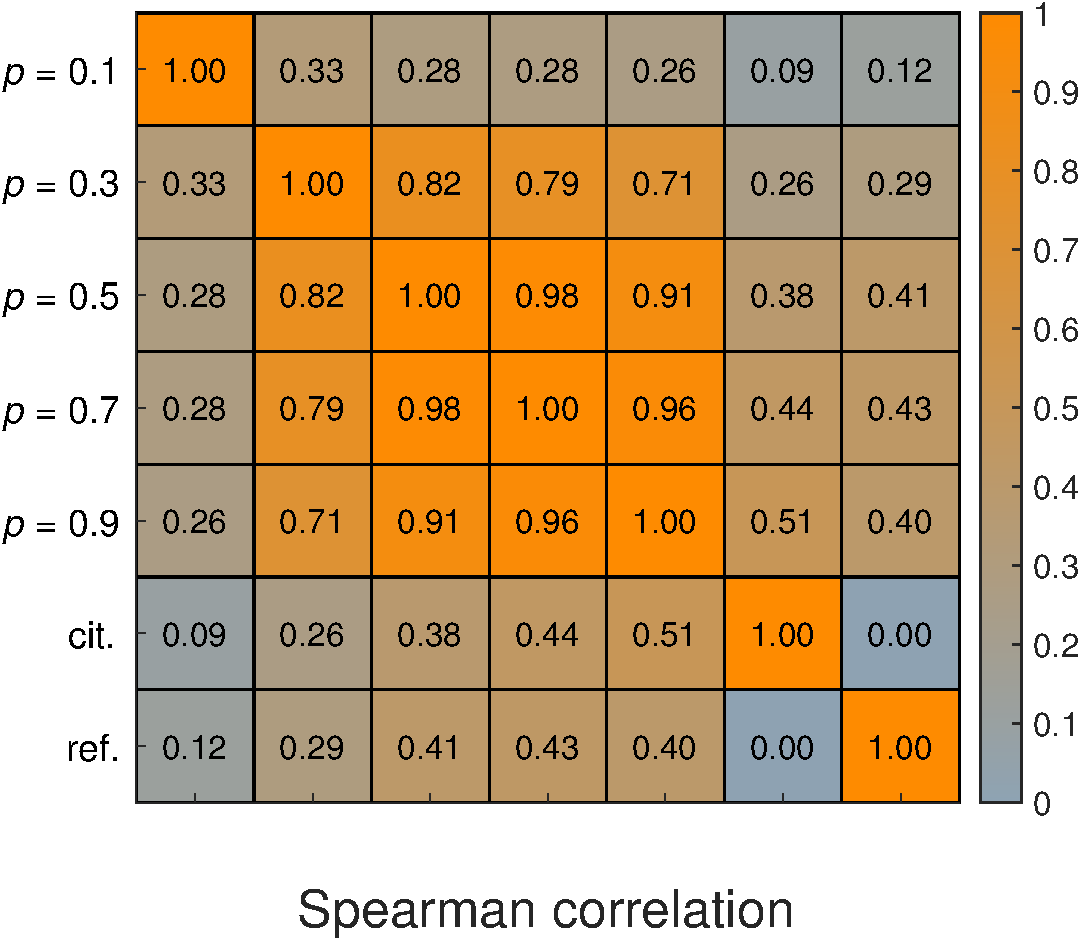
\includegraphics[width=0.425\textwidth]{spearman_Q}\hskip0.05\linewidth
  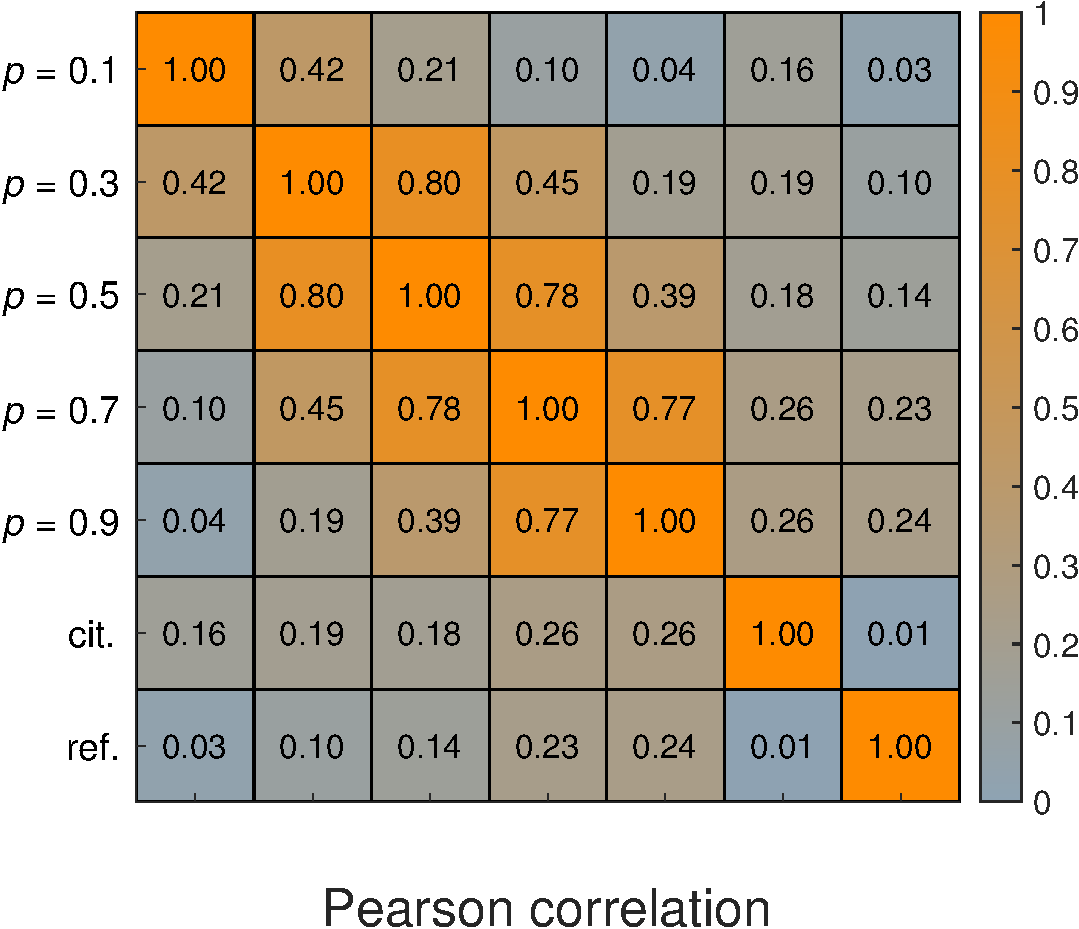
\includegraphics[width=0.425\textwidth]{pearson_Q}
  \caption{High-level results for case 1. \emph{Top left:}~Probability of the existence of an active path between the source and target publications as a function of the parameter $p$. \emph{Top right:}~Cumulative distribution of intermediacy scores for different values of $p$. \emph{Bottom:}~Spearman and Pearson correlations between intermediacy scores (for different values of $p$), citation counts, and reference counts.}
  \label{fig:Q}
\end{figure}

For five different values of the parameter $p$, the top-right plot shows the cumulative distribution of the intermediacy scores of our $n = 64\,223$ publications. As is to be expected, when $p$ is close to zero, intermediacy scores are extremely small. For instance, for $p = 0.1$, almost all intermediacy scores are below $10^{-6}$. On the other hand, when $p$ is getting close to one, intermediacy scores also approach one. For $p = 0.9$, for instance, there are hardly any intermediacy scores below $0.1$.

The matrices in the bottom part of~\figref{Q} provide the correlations between the intermediacy scores obtained for five different values of the parameter $p$. Correlations with citation counts and reference counts are provided as well. (We use the term \emph{citation count} to refer to the number of incoming citation links of a publication, while we use the term \emph{reference count} to refer to the number of outgoing citation links of a publication. Only citation links located on a citation path between the source and target publications are counted.) The left matrix reports Spearman correlations, while the right matrix reports Pearson correlations. We consider intermediacy scores to be most useful from an ordinal (as opposed to a cardinal) perspective. From this point of view, Spearman correlations are more relevant than Pearson correlations, but for completeness we report both types of correlations. The Spearman correlations show that values of $0.3$, $0.5$, $0.7$, and $0.9$ for $p$ all yield fairly similar rankings of publications in terms of intermediacy. However, the ranking obtained for $p = 0.1$ is quite different. Pearson correlations tend to be lower than Spearman correlations. Hence, even when different values of $p$ yield similar rankings of publications, there usually does not exist a clear linear relationship between the intermediacy scores. Finally, regardless of the value of $p$, it turns out that intermediacy scores are not very strongly correlated with citation counts and reference counts.

We now explore our results in more detail. Based on our expert knowledge of the topic under study, we found that the most useful results were obtained by setting the parameter $p$ equal to $0.1$. \tblref{Q} lists the ten publications with the highest intermediacy for $p = 0.1$. For each publication, the intermediacy is reported for five different values of $p$. In addition, the table also reports each publication’s citation count and reference count. The left panel in~\figref{nets} shows the citation network of the ten most intermediate publications for $p = 0.1$.

\begin{sidewaystable}%
  \begin{tabular}{rp{14cm}rrrrrrr}\toprule
    & & \multicolumn{5}{c}{$p$} \\\cmidrule{3-7}
    & & $0.1$ & $0.3$ & $0.5$ & $0.7$ & $0.9$ & cit. & ref. \\\midrule
    $t$ & Newman \& Girvan (2004), Finding and evaluating community structure in networks, {\it Phys.\ Rev.\ E} {\bf 69}(2), 026113. & $0.3010$ & $0.9922$ & $1.0000$ & $1.0000$ & $1.0000$ & $468$ & $0$ \\
    $s$ & Klavans \& Boyack (2017), Which type of citation analysis generates the most accurate taxonomy of scientific and technical knowledge?, {\it J.\ Assoc.\ Inf.\ Sci.\ Tec.} {\bf 68}(4), 984-998. & $0.3010$ & $0.9922$ & $1.0000$ & $1.0000$ & $1.0000$ & $0$ & $24$ \\\midrule
    $1$ & Waltman \& Van Eck (2013), A smart local moving algorithm for large-scale modularity-based community detection, {\it Eur.\ Phys.\ J.\ B} {\bf 86}, 471. & $0.0609$ & $0.3756$ & $0.6558$ & $0.8780$ & $0.9882$ & $2$ & $27$ \\
    $2$ & Waltman \& Van Eck (2012), A new methodology for constructing a publication-level classification system of science, {\it J.\ Assoc.\ Inf.\ Sci.\ Tec.} {\bf 63}(12), 2378-2392. & $0.0600$ & $0.6947$ & $0.9636$ & $0.9988$ & $1.0000$ & $15$ & $22$ \\
    $3$ & Hric et al.\ (2014), Community detection in networks: Structural communities versus ground truth, {\it Phys.\ Rev.\ E} {\bf 90}(6), 062805. & $0.0519$ & $0.2995$ & $0.4992$ & $0.7002$ & $0.8995$ & $1$ & $29$ \\
    $4$ & Fortunato (2010), Community detection in graphs, {\it Phys.\ Rep.} {\bf 486}(3-5), 75-174. & $0.0371$ & $0.6289$ & $0.9719$ & $0.9998$ & $1.0000$ & $73$ & $154$ \\
    $5$ & Newman (2006), Modularity and community structure in networks, {\it P.\ Natl.\ Acad.\ Sci.\ USA} {\bf 103}(23), 8577-8582. & $0.0350$ & $0.7360$ & $0.9789$ & $0.9996$ & $1.0000$ & $221$ & $8$ \\
    $6$ & Ruiz-Castillo \& Waltman (2015), Field-normalized citation impact indicators using algorithmically constructed classification systems of science, {\it J.\ Informetr.} {\bf 9}(1), 102-117. & $0.0239$ & $0.3595$ & $0.6243$ & $0.8474$ & $0.9810$ & $2$ & $24$ \\
    $7$ & Blondel et al.\ (2008), Fast unfolding of communities in large networks, {\it J.\ Stat.\ Mech.}, P10008. & $0.0222$ & $0.8364$ & $0.9978$ & $1.0000$ & $1.0000$ & $78$ & $21$ \\
    $8$ & Newman (2006), Finding community structure in networks using the eigenvectors of matrices, {\it Phys.\ Rev.\ E} {\bf 74}(3), 036104. & $0.0213$ & $0.8505$ & $0.9989$ & $1.0000$ & $1.0000$ & $138$ & $18$ \\
    $9$ & Newman (2004), Fast algorithm for detecting community structure in networks, {\it Phys.\ Rev.\ E} {\bf 69}(6), 066133. & $0.0203$ & $0.2955$ & $0.5011$ & $0.6998$ & $0.9004$ & $246$ & $1$ \\
    $10$ & Rosvall \& Bergstrom (2008), Maps of random walks on complex networks reveal community structure, {\it P.\ Natl.\ Acad.\ Sci.\ USA} {\bf 105}(4), 1118-1123. & $0.0196$ & $0.8033$ & $0.9942$ & $1.0000$ & $1.0000$ & $70$ & $10$ \\\bottomrule
  \end{tabular}
  \caption{Top ten most intermediate publications (for $p = 0.1$) in case 1.}
  \label{tbl:Q}
\end{sidewaystable}

\begin{figure}[t]
  \centering%
  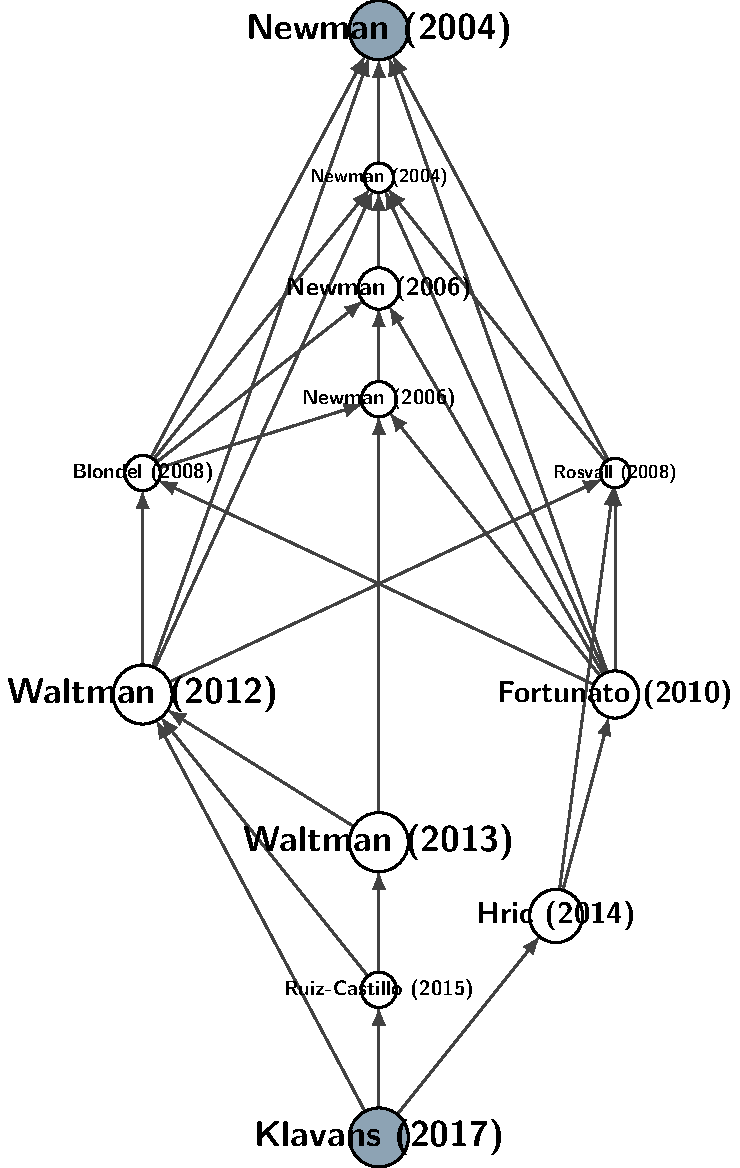
\includegraphics[height=0.575\linewidth]{example_Q}%
  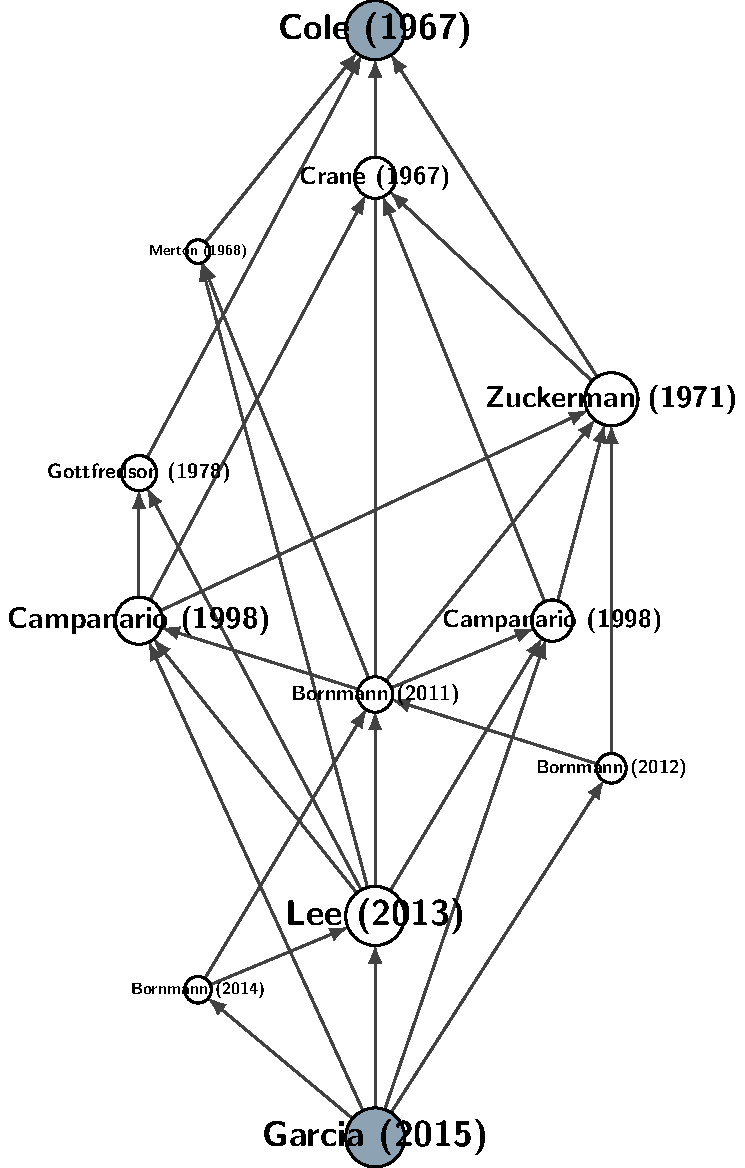
\includegraphics[height=0.575\linewidth]{example_peerrev}
  \caption{Citation network of the top ten most intermediate publications (for $p = 0.1$) in case 1 \emph{(left)} and case 2 \emph{(right)}.}
  \label{fig:nets}
\end{figure}

What do we learn from the results presented in~\tblref{Q} and \figref{nets}? The two publications with the highest intermediacy (Waltman \& Van Eck, 2012, 2013) played a key role in introducing modularity-based approaches in the scientometric community. Waltman and Van Eck (2012) proposed the use of modularity-based approaches for constructing classification systems of scientific publications, while Waltman and Van Eck (2013) introduced an algorithm for implementing these modularity-based approaches. This algorithm can be seen as an improvement of the so-called Louvain algorithm introduced by Blondel et al.\ (2008), which is also among the ten most intermediate publications. Most of the other publications in~\tblref{Q} and \figref{nets} are classical publications on community detection in general and modularity in particular. This applies to the three publications by Newman and also to Rosvall and Bergstrom (2008) and Fortunato (2010). The publications by Newman all deal with modularity-based community detection. Rosvall and Bergstrom (2008) proposed an alternative approach to community detection. They applied their approach to a citation network of scientific journals, which explains the connection with the scientometric literature. Fortunato (2010) is a review of the literature on community detection. The intermediacy of this publication is probably strongly influenced by its large number of references. Hric et al.\ (2014) is a more recent publication on community detection. This publication focuses on the challenges of evaluating the results produced by community detection methods. This issue is very relevant in a scientometric context, and therefore the publication was cited by our source publication (Klavans \& Boyack, 2017). Finally, there is one more scientometric publication in~\tblref{Q} and \figref{nets}. This publication (Ruiz-Castillo \& Waltman, 2015) is one of the first studies presenting a scientometric application of classification systems of scientific publications constructed using a modularity-based approach. The publication was also cited by our source publication.

The citation counts reported in~\tblref{Q} show that some publications, especially the more recent ones, have a high intermediacy even though they have been cited only a very limited number of times. This makes clear that a ranking of publications based on intermediacy is quite different from a citation-based ranking of publications. The publications in~\tblref{Q} that have a high intermediacy and a small number of citations do have a substantial number of references.

\subsection{\label{sec:pr}Case 2: Peer review}

We now turn to our second case, in which we analyze the literature on peer review. The second case is based on data from the Web of Science database. We make use of the same data that was also used in a recent paper by~\citet{Batagelj2017}. The authors of this paper kindly made their data available to us.

We started with a citation network of $45\,965$ publications dealing with peer review. This is the citation network that was labeled CiteAcy by~\citet{Batagelj2017}. We selected Cole and Cole (1967) and Garcia et al.\ (2015) as our target and source publications. The main path analysis carried out by~\citet{Batagelj2017} suggests that these are central publications in the literature on peer review. For the purpose of our analysis, only publications located on a citation path between our source and target publications are of relevance. Other publications play no role in the analysis. We therefore restricted the analysis to the $n = 615$ publications located on a citation path from Garcia et al.\ (2015) to Cole and Cole (1967). These publications turned out to be connected by $m = 3\,420$ citation links, resulting in an average of $k = 2m / n = 11.12$ citation links per publication. Like in the first case discussed above, our Monte Carlo algorithm was used to calculate intermediacy scores for different values of the parameter $p$.

\figref{pr} presents high-level results. These results are quite similar to the corresponding results for our first case, presented in~\figref{Q}. As can be seen in the top-left plot, the rule of thumb from percolation theory yields $p = 1 / k = 0.09$, which is close to the value of $0.11$ obtained in our first case. However, the probability of the existence of an active path between the source and target publications equals $0.03$, which is much lower than the probability of $0.40$ in our first case. Furthermore, intermediacy scores tend to be higher in our second case than in our first case. This can be seen by comparing the top-right plot in~\figref{pr} to the corresponding plot in~\figref{Q}. We note that the former plot has a linear horizontal axis, while the horizontal axis in the latter plot is logarithmic.

\begin{figure}[t]
  \centering%
  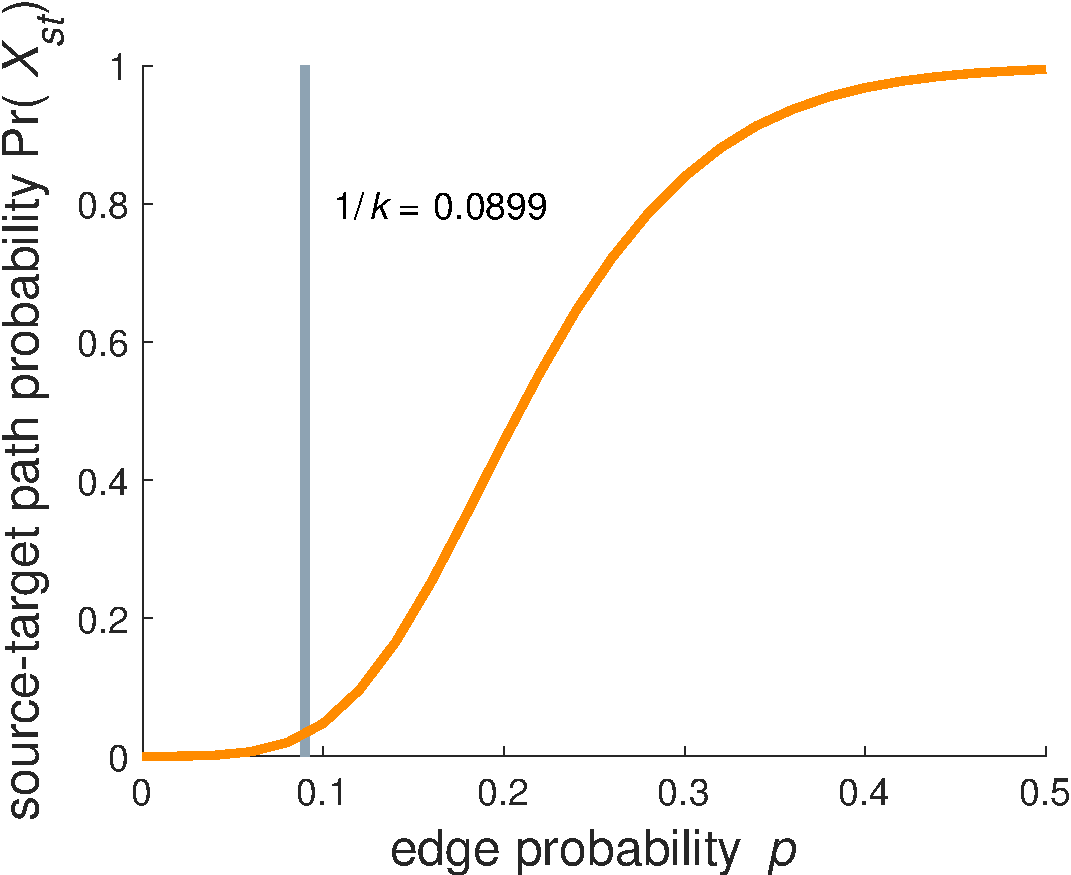
\includegraphics[width=0.4\textwidth]{phist_peerrev}\hskip0.075\linewidth
  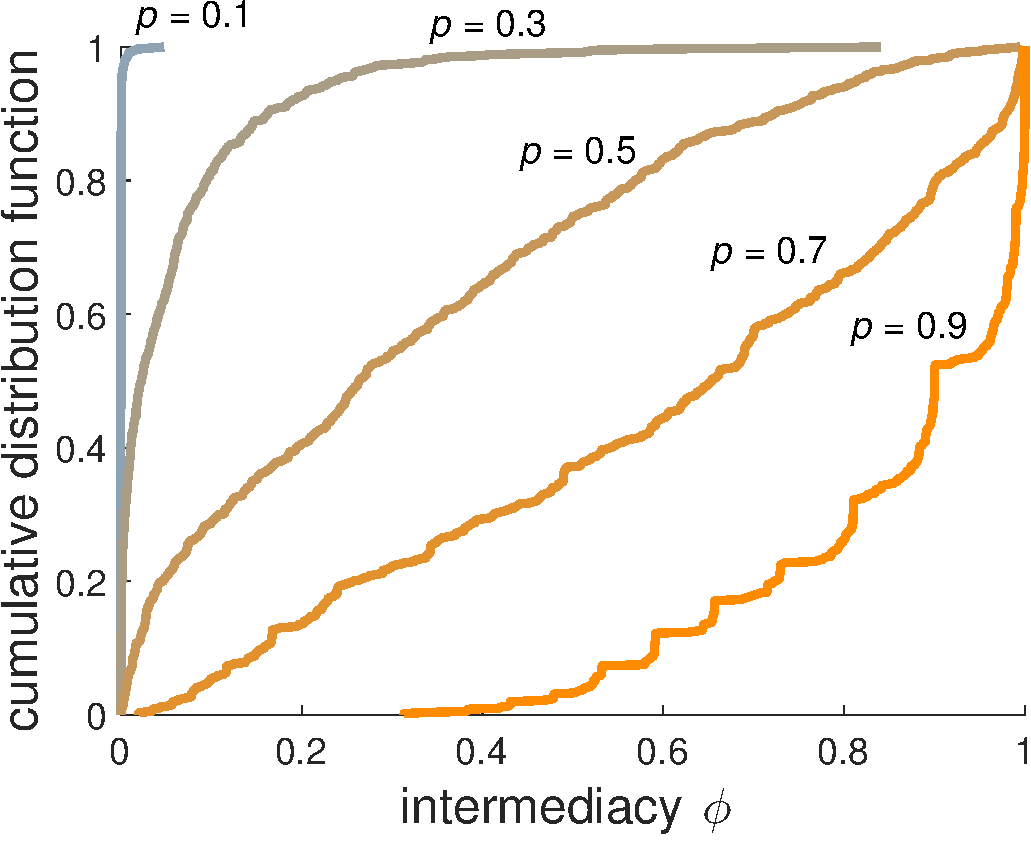
\includegraphics[width=0.4\textwidth]{distributions_peerrev}\\\vskip0.05\linewidth
  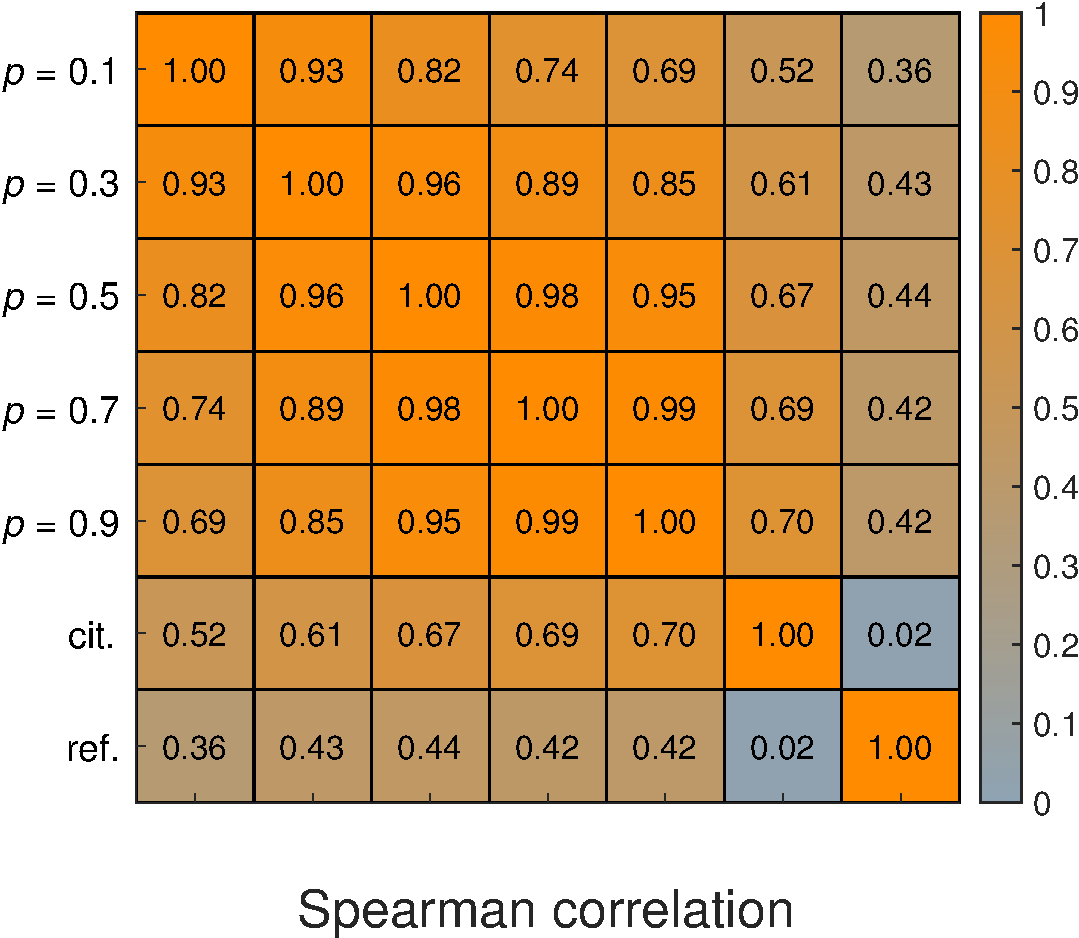
\includegraphics[width=0.425\textwidth]{spearman_peerrev}\hskip0.05\linewidth
  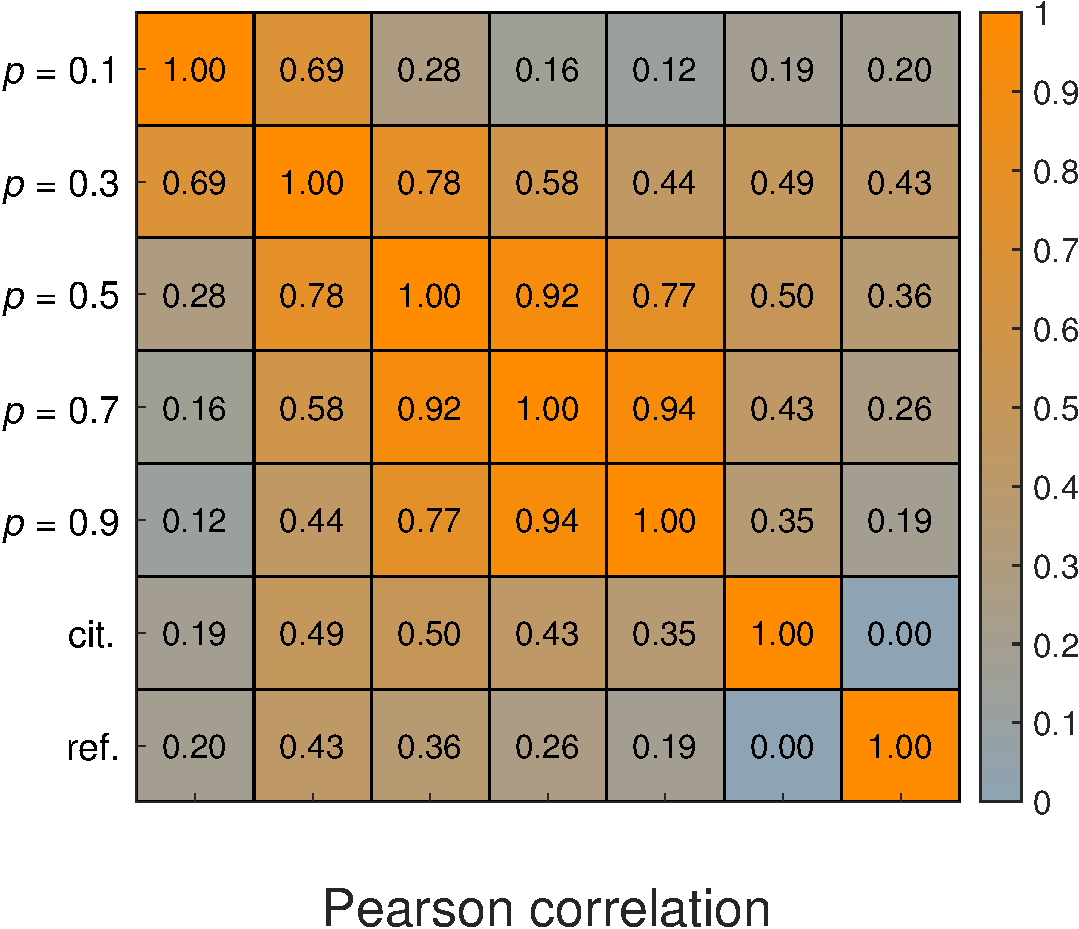
\includegraphics[width=0.425\textwidth]{pearson_peerrev}
  \caption{High-level results for case 2. \emph{Top left:} Probability of the existence of an active path between the source and target publications as a function of the parameter $p$. \emph{Top right:} Cumulative distribution of intermediacy scores for different values of $p$. \emph{Bottom:} Spearman and Pearson correlations between intermediacy scores (for different values of $p$), citation counts, and reference counts.}
  \label{fig:pr}
\end{figure}

\tblref{pr} lists the ten publications with the highest intermediacy, where we use a value of $0.1$ for the parameter $p$, just like in~\tblref{Q}. The right panel in~\figref{nets} shows the citation network of the ten most intermediate publications. There are numerous paths in this citation network going from our source publication (Garcia et al., 2015) to our target publication (Cole \& Cole, 1967). We regard these paths as the core paths between the source and target publications.

\begin{sidewaystable}%
  \begin{tabular}{rp{14cm}rrrrrrr}\toprule
    & & \multicolumn{5}{c}{$p$} \\\cmidrule{3-7}
    & & $0.1$ & $0.3$ & $0.5$ & $0.7$ & $0.9$ & cit. & ref. \\\midrule
    $t$ & Cole \& Cole (1967), Scientific output and recognition: A study in the operation of the reward system in science, {\it Am.\ Sociol.\ Rev.} {\bf 32}(3), 377-390. & $0.0475$ & $0.8405$ & $0.9946$ & $0.9999$ & $1.0000$ & $14$ & $0$ \\
    $s$ & Garcia et al.\ (2015), The author-editor game, {\it Scientometrics} {\bf 104}(1), 361-380. & $0.0475$ & $0.8405$ & $0.9946$ & $0.9999$ & $1.0000$ & $0$ & $8$ \\\midrule
    $1$ & Lee et al.\ (2013), Bias in peer review, {\it J.\ Assoc.\ Inf.\ Sci.\ Tec.} {\bf 64}(1), 2-17. & $0.0184$ & $0.5103$ & $0.8652$ & $0.9858$ & $0.9999$ & $5$ & $71$ \\
    $2$ & Zuckerman \& Merton (1971), Patterns of evaluation in science: Institutionalisation, structure and functions of the referee system, {\it Minerva} {\bf 9}(1), 66-100. & $0.0160$ & $0.3359$ & $0.6221$ & $0.8468$ & $0.9812$ & $73$ & $2$ \\
    $3$ & Campanario (1998), Peer review for journals as it stands today: Part 1, {\it Sci.\ Commun.} {\bf 19}(3), 181-211. & $0.0126$ & $0.5916$ & $0.9673$ & $0.9993$ & $1.0000$ & $23$ & $35$ \\
    $4$ & Crane (1967), The gatekeepers of science: Some factors affecting the selection of articles for scientific journals, {\it Am.\ Sociol.} {\bf 2}(4), 195-201. & $0.0092$ & $0.2700$ & $0.4982$ & $0.7000$ & $0.8998$ & $34$ & $1$ \\
    $5$ & Campanario (1998), Peer review for journals as it stands today: Part 2, {\it Sci.\ Commun.} {\bf 19}(4), 277-306. & $0.0090$ & $0.5170$ & $0.9521$ & $0.9985$ & $1.0000$ & $15$ & $30$ \\
    $6$ & Gottfredson (1978), Evaluating psychological research reports: Dimensions, reliability, and correlates of quality judgments, {\it Am.\ Psychol.} {\bf 33}(10), 920-934. & $0.0083$ & $0.3199$ & $0.6220$ & $0.8466$ & $0.9808$ & $26$ & $2$ \\
    $7$ & Bornmann (2011), Scientific peer review, {\it Annu.\ Rev.\ Inform.\ Sci.} {\bf 45}(1), 197-245. & $0.0079$ & $0.3333$ & $0.7762$ & $0.9748$ & $0.9999$ & $6$ & $71$ \\
    $8$ & Bornmann (2012), The Hawthorne effect in journal peer review, {\it Scientometrics} {\bf 91}(3), 857-862. & $0.0071$ & $0.2593$ & $0.4995$ & $0.7001$ & $0.9002$ & $1$ & $20$ \\
    $9$ & Bornmann (2014), Do we still need peer review? An argument for change, {\it J.\ Assoc.\ Inf.\ Sci.\ Tec.} {\bf 65}(1), 209-213. & $0.0068$ & $0.2745$ & $0.4999$ & $0.6998$ & $0.9002$ & $1$ & $17$ \\
    $10$ & Merton (1968), The Matthew effect in science, {\it Science} {\bf 159}(3810), 56-63. & $0.0051$ & $0.2431$ & $0.4969$ & $0.7006$ & $0.9005$ & $29$ & $1$ \\\bottomrule
  \end{tabular}
  \caption{Top ten most intermediate publications (for $p = 0.1$) in case 2.}
  \label{tbl:pr}
\end{sidewaystable}

Since our knowledge of the literature on peer review is limited, we do not provide an interpretation of the results obtained using intermediacy. Instead, we compare these results to results produced by main path analysis. More specifically, we compare the core paths shown in the right panel in~\figref{nets} to the results obtained by~\citet{Batagelj2017} using main path analysis. Different variants of main path analysis were used by~\citet{Batagelj2017}. Both using the original version of main path analysis~\cite{Hummon1989} and using a more recent variant~\cite{Liu2012}, the paths that were identified were rather lengthy, as can be seen in Figs.~9 and~10 in~\citet{Batagelj2017}. The shortest paths still included about $20$ publications. This confirms the fundamental difference identified in~\secref{intermediacy} between intermediacy and main path analysis. Main path analysis tends to favor longer paths over shorter ones, whereas intermediacy has the opposite tendency.

% % % % % % % % % % % % % % % % % % % % % % % % % % 
%
%				CONCLUSIONS
%
% % % % % % % % % % % % % % % % % % % % % % % % % %

\section{\label{sec:conclusions}Conclusions}

\redo{In conclusion, we have introduced a novel way of defining the importance of publications in the development between two publications.
We call this the \emph{intermediacy} of publications with respect to a source and target publication.
We have introduced an exact algorithm that is suitable for relatively small citation networks.
For analysing larger networks, we rely on a simple Monte Carlo algorithm.}

\redo{Theoretical analysis of intermediacy shows that the failure probability $q$ interpolates between two extremes.
When $q=0$ the ranking of intermediacy is dominated by the number of edge independent paths.
When $q=1$ the ranking of intermediacy is dominated by the shortest path length.
Empirical case studies reveal that the intermediacy is quite different from the number of citations.}

\redo{Several possible extensions of our method are possible.
It could be of interest for example to exclude publications with a certain probability, rather than citations.
Similarly, we could look at the probability that a citation is on the path between the source and the target, rather than a publication.}

% % % % % % % % % % % % % % % % % % % % % % % % % % 
%
%				BIBLIOGRAPHY
%
% % % % % % % % % % % % % % % % % % % % % % % % % %

\bibliographystyle{unsrtnat}
\bibliography{bibliography}

\end{document}
